% cloudforger_reference.tex
% Developer reference guide for the src/cloudforger package.
% Compile with: pdflatex cloudforger_reference.tex
% All packages are part of standard TeX Live / MiKTeX distributions.

\documentclass[11pt, a4paper]{article}

%% ── Encoding & fonts ────────────────────────────────────────────────────────
\usepackage[T1]{fontenc}
\usepackage[utf8]{inputenc}
\usepackage{lmodern}
\usepackage{microtype}

%% ── Page geometry ───────────────────────────────────────────────────────────
\usepackage[margin=2.5cm, top=3cm, bottom=3cm]{geometry}

%% ── Colour ──────────────────────────────────────────────────────────────────
\usepackage[dvipsnames, svgnames]{xcolor}
\definecolor{codebg}{HTML}{F5F5F5}
\definecolor{keywordcol}{HTML}{0033CC}
\definecolor{commentcol}{HTML}{559955}
\definecolor{stringcol}{HTML}{CC3300}
\definecolor{identcol}{HTML}{000000}
\definecolor{linkblue}{HTML}{1A4999}
\definecolor{headercol}{HTML}{2C3E6B}

%% ── Hyperlinks ──────────────────────────────────────────────────────────────
\usepackage[colorlinks=true, linkcolor=linkblue,
            urlcolor=linkblue, citecolor=linkblue,
            bookmarksnumbered=true]{hyperref}

%% ── Mathematics ─────────────────────────────────────────────────────────────
\usepackage{amsmath, amssymb}

%% ── Tables ──────────────────────────────────────────────────────────────────
\usepackage{booktabs}
\usepackage{array}
\usepackage{tabularx}
\usepackage{longtable}

%% ── Compact list spacing ────────────────────────────────────────────────────
\setlength{\topsep}{2pt}
\setlength{\itemsep}{1pt}
\setlength{\parsep}{0pt}

%% ── Code listings ───────────────────────────────────────────────────────────
\usepackage{listings}

\lstdefinestyle{pycode}{
  language=Python,
  backgroundcolor=\color{codebg},
  basicstyle=\ttfamily\small,
  keywordstyle=\bfseries\color{keywordcol},
  commentstyle=\itshape\color{commentcol},
  stringstyle=\color{stringcol},
  identifierstyle=\color{identcol},
  showstringspaces=false,
  breaklines=true,
  breakatwhitespace=false,
  frame=single,
  framerule=0.5pt,
  rulecolor=\color{gray!60},
  xleftmargin=1em,
  xrightmargin=0.5em,
  aboveskip=6pt,
  belowskip=6pt,
  tabsize=4,
  morekeywords={None, True, False, dataclass, abstractmethod, property,
                np, torch, nn, ABC},
  literate={|}{{{\color{keywordcol}|}}}{1},
}
\lstset{style=pycode}

%% ── TikZ ────────────────────────────────────────────────────────────────────
\usepackage{tikz}
\usetikzlibrary{arrows.meta, shapes.geometric, shapes.misc,
                positioning, fit, backgrounds, calc, shadows}

%% ── Spacing ─────────────────────────────────────────────────────────────────
\usepackage{parskip}
\setlength{\parskip}{6pt}

%% ── Paragraph helper ────────────────────────────────────────────────────────
\usepackage{ragged2e}

%% ── Misc ────────────────────────────────────────────────────────────────────
\usepackage{graphicx}
\usepackage{float}

%% ── Convenience macros ──────────────────────────────────────────────────────
\newcommand{\code}[1]{\texttt{#1}}
\newcommand{\pyfile}[1]{\texttt{\small #1}}
\newcommand{\typename}[1]{\textbf{\texttt{#1}}}
\newcommand{\param}[2]{\texttt{#1}\;(\textit{#2})}
\newcommand{\note}[1]{\textit{\color{gray!70!black}#1}}

%% ─────────────────────────────────────────────────────────────────────────────
\title{\LARGE\bfseries\color{headercol}%
  \texttt{cloudforger} Developer Reference\\[0.4em]
  \large\normalfont\color{gray!80!black}%
  A guide to the \texttt{src/cloudforger} package
}
\author{Auto-generated from source}
\date{June 2026}
%% ─────────────────────────────────────────────────────────────────────────────

\begin{document}

\maketitle
\thispagestyle{empty}

\vspace{1em}
\begin{abstract}
\noindent
This document is the authoritative developer reference for the
\code{cloudforger} Python package located at \pyfile{src/cloudforger/}
within the \emph{point-process-tda} research project.
It covers every public class and function, the end-to-end data pipeline
(from process simulation to neural-network training), and a minimal
worked example that a new contributor can run immediately.
All content is derived directly from the source code; nothing is
assumed or invented.
\end{abstract}

\newpage
\tableofcontents
\newpage

%% ═══════════════════════════════════════════════════════════════════════════
\section{Package Overview}
\label{sec:overview}
%% ═══════════════════════════════════════════════════════════════════════════

\subsection{Purpose and Scope}

\code{cloudforger} is a research-grade Python library for generating
spatial point clouds from classical stochastic point processes,
computing topological and statistical descriptors of those clouds,
and routing the resulting feature representations into PyTorch neural
networks for classification or parameter estimation.

The package sits inside the broader \emph{point-process-tda} project,
which investigates whether topological data analysis (TDA) features
can distinguish point-process types across varying ambient dimensions.
\code{cloudforger} is the computational engine; the surrounding
\pyfile{scripts/} directory contains the experiment runners and
processing scripts that orchestrate it.

\subsection{Package Layout}

\begin{center}
\begin{tabular}{ll}
\toprule
\textbf{Subpackage / file} & \textbf{Responsibility} \\
\midrule
\code{core/}            & Shared data structures (\code{PointCloud}, \code{Region},
                          \code{PersistenceDiagram}, \code{CorrelationFeatures}) \\
\code{processes/}       & Point-process implementations (Poisson, Thomas, Matérn II) \\
\code{stats/}           & Empirical summary statistics (pair-distance CDF) \\
\code{tda/filtration/}  & Persistent-homology computation (Rips filtration) \\
\code{tda/vectorizer/}  & Diagram-to-image vectorization (persistence images) \\
\code{tda/calibration.py} & Automatic bound selection for vectorizers \\
\code{nn/data.py}       & PyTorch \code{Dataset} wrappers \\
\code{nn/encoders/}     & Modality-specific neural encoders \\
\code{nn/heads/}        & Task heads (classification, parameter estimation) \\
\code{nn/models/}       & Assembled model wrappers (\code{Single-} / \code{MultiModalModel}) \\
\code{nn/train.py}      & Training and evaluation loop functions \\
\code{nn/splits.py}     & Reproducible train/val/test splitting \\
\bottomrule
\end{tabular}
\end{center}

\subsection{Key External Dependencies}

\begin{center}
\begin{tabular}{ll}
\toprule
\textbf{Package} & \textbf{Role} \\
\midrule
\code{numpy}        & Array arithmetic and seeded random number generation \\
\code{scipy}        & \code{cKDTree} for nearest-neighbour queries (Matérn process) \\
\code{ripser}       & Efficient Vietoris--Rips persistent homology \\
\code{torch}        & Tensor computation, neural networks, datasets \\
\code{pickle / yaml}& Dataset serialization and configuration loading \\
\bottomrule
\end{tabular}
\end{center}

%% ═══════════════════════════════════════════════════════════════════════════
\section{Core Data Structures}
\label{sec:datastructs}
%% ═══════════════════════════════════════════════════════════════════════════

\subsection{\typename{Region} and \typename{Box}}
\label{subsec:region}
\pyfile{src/cloudforger/core/region.py}

\typename{Region} is an abstract base class representing a spatial domain.
Every point process samples exclusively within a \code{Region}.

\begin{lstlisting}
class Region(ABC):
    @property
    @abstractmethod
    def dimension(self) -> int: ...

    @property
    @abstractmethod
    def volume(self) -> float: ...

    @abstractmethod
    def contains(self, point: np.ndarray) -> np.ndarray: ...
    # Returns boolean mask of shape (N,)

    @abstractmethod
    def sample_uniform(self, n: int,
                       rng: np.random.Generator) -> np.ndarray: ...
    # Returns (n, dimension) array

    @abstractmethod
    def expanded(self, pad: float) -> "Region": ...
    # Returns a new Region grown by `pad` on every side
\end{lstlisting}

\typename{Box} is the only concrete implementation.
It represents an axis-aligned hyperrectangle $[\mathbf{l}, \mathbf{h}]^d$
defined by two 1-D numpy arrays \code{low} and \code{high}.

\begin{lstlisting}
class Box(Region):
    def __init__(self, low: np.ndarray, high: np.ndarray):
        # low < high required element-wise; both must be 1-D
        ...
    # volume = prod(high - low)
    # contains uses >= low and <= high (closed box)
    # expanded(pad) returns Box(low - pad, high + pad)
\end{lstlisting}

\textbf{Usage example:}
\begin{lstlisting}
import numpy as np
from cloudforger.core.region import Box

# Unit square in 2-D
region = Box(low=np.zeros(2), high=np.ones(2))
print(region.volume)    # 1.0
print(region.dimension) # 2
\end{lstlisting}

\subsection{\typename{PointCloud}}
\label{subsec:pointcloud}
\pyfile{src/cloudforger/core/cloud.py}

The central data structure of the package.
It bundles raw point coordinates with provenance metadata.

\begin{center}
\begin{tabular}{lll}
\toprule
\textbf{Field} & \textbf{Type} & \textbf{Description} \\
\midrule
\code{points}           & \code{np.ndarray}  & Shape $(N, D)$ --- coordinates of $N$ points in $D$ dimensions \\
\code{generator\_name}  & \code{str}         & Name of the process that produced this cloud \\
\code{generator\_params}& \code{dict}        & Process hyperparameters at sampling time \\
\code{seed}             & \code{int | None}  & RNG seed for reproducibility \\
\code{region}           & \code{Region | None} & Sampling domain (required by some statistics) \\
\midrule
\code{n\_points}  & \code{int} & \emph{(property)} \code{points.shape[0]} \\
\code{dimension}  & \code{int} & \emph{(property)} \code{points.shape[1]} \\
\bottomrule
\end{tabular}
\end{center}

\code{PointCloud} is a \code{@dataclass}; all fields are stored as-is
(no copies made).

\begin{lstlisting}
from cloudforger.core.cloud import PointCloud
import numpy as np

pts = np.random.rand(200, 3)
cloud = PointCloud(
    points=pts,
    generator_name="example",
    generator_params={},
    seed=42,
)
print(cloud)
# PointCloud(n=200, d=3, generator='example', seed=42)
\end{lstlisting}

\subsection{\typename{PointProcess}}
\label{subsec:pointprocess}
\pyfile{src/cloudforger/core/base.py}

Abstract base class that all point processes extend.
Subclasses must implement \code{name}, \code{params},
and the internal sampling method \code{\_sample\_points}.
The \textbf{public API} is the single method \code{sample()}.

\begin{lstlisting}
class PointProcess(ABC):
    @property
    @abstractmethod
    def name(self) -> str: ...

    @property
    @abstractmethod
    def params(self) -> dict[str, Any]: ...

    @abstractmethod
    def _sample_points(self, n: int, region: Region,
                       rng: np.random.Generator) -> np.ndarray: ...

    def sample(self, n: int, region: Region,
               seed: int | None = None) -> PointCloud:
        rng = np.random.default_rng(seed)
        points = self._sample_points(n, region, rng)
        return PointCloud(points=points,
                          generator_name=self.name,
                          generator_params=self.params,
                          seed=seed,
                          region=region)
\end{lstlisting}

The argument \code{n} carries different semantics depending on the
subclass --- it may be the exact output count (Poisson without
intensity) or an unused nominal target (Thomas / Matérn produce a
random count regardless).  See Section~\ref{sec:processes} for details.

\subsection{\typename{PersistenceDiagram}}
\label{subsec:diagram}
\pyfile{src/cloudforger/core/diagram.py}

Stores the output of a persistent-homology computation.

\begin{center}
\begin{tabular}{lll}
\toprule
\textbf{Field} & \textbf{Type} & \textbf{Description} \\
\midrule
\code{diagrams}           & \code{dict[int, np.ndarray]} & Maps homology dimension $k$ to an array of shape $(M_k, 2)$ of birth--death pairs \\
\code{generator\_name}    & \code{str}                   & Provenance: process that produced the source cloud \\
\code{generator\_params}  & \code{dict}                  & Process parameters \\
\code{seed}               & \code{int | None}            & RNG seed \\
\code{filtration\_name}   & \code{str}                   & Filtration type (e.g.\ \code{"rips"}) \\
\code{filtration\_params} & \code{dict}                  & Filtration parameters \\
\midrule
\code{dimensions()} & \code{list[int]} & \emph{(method)} Sorted list of stored homology dimensions \\
\code{finite\_pairs(dim)} & \code{np.ndarray} & \emph{(method)} Pairs with both birth \emph{and} death finite \\
\bottomrule
\end{tabular}
\end{center}

Death values of $+\infty$ (i.e.\ the feature never dies) are present in
raw \code{ripser} output; \code{finite\_pairs(dim)} removes them.

\subsection{\typename{CorrelationFeatures}}
\label{subsec:corrfeatures}
\pyfile{src/cloudforger/core/features.py}

Wraps the output of a \code{CloudStatistic} computation.

\begin{center}
\begin{tabular}{lll}
\toprule
\textbf{Field} & \textbf{Type} & \textbf{Description} \\
\midrule
\code{features}           & \code{dict[str, np.ndarray]} & Maps statistic name to its 1-D feature vector \\
\code{generator\_name}    & \code{str}                   & Source process name \\
\code{generator\_params}  & \code{dict}                  & Source process parameters \\
\code{seed}               & \code{int | None}            & RNG seed \\
\code{statistic\_params}  & \code{dict}                  & Parameters of the computing statistic \\
\midrule
\code{names()} & \code{list[str]} & \emph{(method)} Sorted statistic names \\
\code{vector(names)} & \code{np.ndarray} & \emph{(method)} Concatenation of vectors for the given names (all if \code{None}) \\
\bottomrule
\end{tabular}
\end{center}

%% ═══════════════════════════════════════════════════════════════════════════
\section{Point Processes}
\label{sec:processes}
%% ═══════════════════════════════════════════════════════════════════════════

\subsection{\typename{PoissonProcess}}
\pyfile{src/cloudforger/processes/poisson.py}

\begin{lstlisting}
class PoissonProcess(PointProcess):
    def __init__(self, intensity: float | None = None):
        ...
\end{lstlisting}

\textbf{Two modes} depending on whether \code{intensity} is supplied:

\begin{itemize}
  \item \textbf{Conditional mode} (\code{intensity=None}):
        Samples exactly \code{n} points uniformly at random in the region.
        This is the conditional Poisson process given count $n$.
  \item \textbf{Homogeneous mode} (\code{intensity=}\(\lambda > 0\)):
        Draws a random count $N \sim \mathrm{Poisson}(\lambda \cdot |W|)$
        and then places $N$ points uniformly in the region $W$.
\end{itemize}

The parameter name in \code{params} is \code{"intensity"};
the process name is \code{"poisson"}.

\subsection{\typename{ThomasProcess}}
\pyfile{src/cloudforger/processes/thomas.py}

The Thomas process (Neyman--Scott with Gaussian scatter kernel)
generates clustered patterns.

\begin{lstlisting}
class ThomasProcess(PointProcess):
    def __init__(self,
                 parent_intensity: float,  # lambda_p > 0
                 mean_offspring:   float,  # mu > 0
                 cluster_scale:    float): # sigma > 0
        ...
\end{lstlisting}

\textbf{Sampling algorithm (edge-corrected):}
\begin{enumerate}
  \item Expand the sampling region by $4\sigma$ on every side to create
        an enlarged guard region.
  \item Sample $N_p \sim \mathrm{Poisson}(\lambda_p \cdot |W_{\mathrm{expanded}}|)$
        parent centres uniformly in the enlarged region.
  \item For each parent $i$, draw offspring count
        $K_i \sim \mathrm{Poisson}(\mu)$.
  \item Scatter offspring around each parent:
        $\mathbf{x}_{ij} = \mathbf{c}_i + \boldsymbol{\epsilon}_{ij}$,
        where $\boldsymbol{\epsilon}_{ij} \sim \mathcal{N}(\mathbf{0},
        \sigma^2 \mathbf{I})$.
  \item Retain only offspring that fall inside the \emph{original} region.
\end{enumerate}

The guard region ensures that offspring landing inside the original
region from parents located just outside it are correctly simulated.
The process name is \code{"thomas"}.

\subsection{\typename{MaternHardCoreProcess} (Type II)}
\pyfile{src/cloudforger/processes/matern.py}

Produces repulsive (inhibitory) patterns via dependent thinning.

\begin{lstlisting}
class MaternHardCoreProcess(PointProcess):
    def __init__(self,
                 parent_intensity: float,  # lambda_p > 0
                 hardcore_radius:  float): # r > 0
        ...
\end{lstlisting}

\textbf{Sampling algorithm:}
\begin{enumerate}
  \item Sample a parent Poisson process with intensity
        $\lambda_p$ in the region.
  \item Assign independent uniform marks $u_i \sim \mathrm{Uniform}(0,1)$
        to every parent.
  \item Build a $k$-d tree over the parent locations.
  \item Retain point $i$ if and only if \emph{no} neighbour within
        distance $r$ has a strictly smaller mark than $u_i$.
\end{enumerate}

This is the Type~II construction; retained points are guaranteed to be
mutually at distance $> r$.  The process name is \code{"matern\_ii"}.

%% ═══════════════════════════════════════════════════════════════════════════
\section{Cloud Generation Pipeline}
\label{sec:pipeline}
%% ═══════════════════════════════════════════════════════════════════════════

\subsection{End-to-End Data Flow}

Figure~\ref{fig:pipeline} shows the complete journey from process
parameters to neural-network inputs, as implemented in the
\pyfile{scripts/} directory using the \code{cloudforger} primitives.

\begin{figure}[H]
\centering
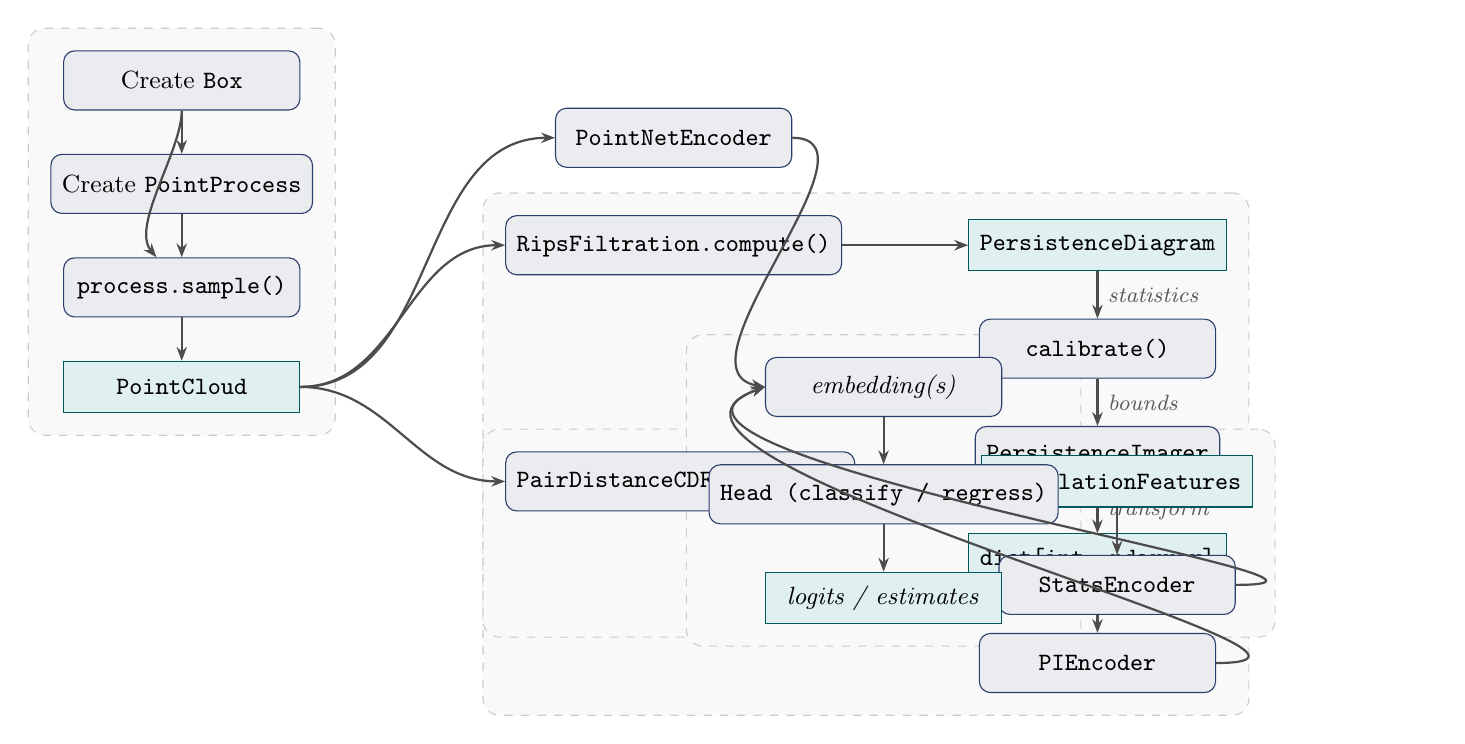
\begin{tikzpicture}[
  node distance=0.55cm and 1.8cm,
  every node/.style={font=\small},
  process/.style={
    rectangle, rounded corners=4pt,
    draw=headercol, fill=headercol!10,
    minimum width=3.0cm, minimum height=0.75cm,
    text centered, inner sep=4pt
  },
  data/.style={
    rectangle,
    draw=Teal!70!black, fill=Teal!12,
    minimum width=3.0cm, minimum height=0.65cm,
    text centered, inner sep=4pt
  },
  arrow/.style={-{Stealth[length=5pt]}, thick, color=gray!60!black},
  label/.style={font=\footnotesize\itshape, text=gray!70!black},
  groupbox/.style={draw=gray!40, dashed, rounded corners=6pt,
                   fill=gray!5, inner sep=8pt}
]

%% ─── Column 1: Generation ───────────────────────────────────────────────────
\node[process] (box)     {Create \texttt{Box}};
\node[process, below=of box] (proc)    {Create \texttt{PointProcess}};
\node[process, below=of proc] (sample)  {\texttt{process.sample()}};
\node[data,    below=of sample] (cloud)   {\texttt{PointCloud}};

\draw[arrow] (box)    -- (proc)   node[midway, right, label] {};
\draw[arrow] (proc)   -- (sample);
\draw[arrow] (sample) -- (cloud);
\draw[arrow] (box)    to[out=-90, in=130, looseness=0.7] (sample);

%% ─── Branch split ────────────────────────────────────────────────────────────
\node[process, right=2.6cm of cloud, yshift=1.8cm] (rips)
      {\texttt{RipsFiltration.compute()}};
\node[process, right=2.6cm of cloud, yshift=-1.2cm] (cdf)
      {\texttt{PairDistanceCDF.compute()}};

\draw[arrow] (cloud.east) to[out=0, in=180] (rips.west);
\draw[arrow] (cloud.east) to[out=0, in=180] (cdf.west);

%% ─── TDA branch ─────────────────────────────────────────────────────────────
\node[data,    right=1.6cm of rips] (dgm)  {\texttt{PersistenceDiagram}};
\node[process, below=0.6cm of dgm]  (cal)  {\texttt{calibrate()}};
\node[process, below=0.6cm of cal]  (img)  {\texttt{PersistenceImager}};
\node[data,    below=0.6cm of img]  (imgs) {\texttt{dict[int, ndarray]}};
\node[process, below=0.6cm of imgs] (pienc){\texttt{PIEncoder}};

\draw[arrow] (rips) -- (dgm);
\draw[arrow] (dgm)  -- (cal) node[midway, right, label] {statistics};
\draw[arrow] (cal)  -- (img) node[midway, right, label] {bounds};
\draw[arrow] (img)  -- (imgs) node[midway, right, label] {transform};
\draw[arrow] (imgs) -- (pienc);

%% ─── Stats branch ────────────────────────────────────────────────────────────
\node[data,    right=1.6cm of cdf] (feat)  {\texttt{CorrelationFeatures}};
\node[process, below=0.6cm of feat] (senc)  {\texttt{StatsEncoder}};

\draw[arrow] (cdf)  -- (feat);
\draw[arrow] (feat) -- (senc);

%% ─── Raw PC branch (dashed) ─────────────────────────────────────────────────
\node[process, above=0.6cm of rips] (pcenc)
      {\texttt{PointNetEncoder}};
\draw[arrow] (cloud.east) to[out=0, in=180] (pcenc.west);

%% ─── Fusion & head ───────────────────────────────────────────────────────────
\node[process, right=5.9cm of cloud] (embed)   {\textit{embedding(s)}};
\node[process, below=0.6cm of embed] (head)    {\texttt{Head (classify / regress)}};
\node[data,    below=0.6cm of head]  (output)  {\textit{logits / estimates}};

\draw[arrow] (pcenc.east)  to[out=0, in=170] (embed.west);
\draw[arrow] (pienc.east)  to[out=0, in=200] (embed.west);
\draw[arrow] (senc.east)   to[out=0, in=200] (embed.west);
\draw[arrow] (embed) -- (head);
\draw[arrow] (head)  -- (output);

%% ─── Background group labels ─────────────────────────────────────────────────
\begin{scope}[on background layer]
  \node[groupbox, fit=(box)(proc)(sample)(cloud),
        label={[font=\footnotesize\bfseries, text=headercol]above:Generation}] {};
  \node[groupbox, fit=(rips)(dgm)(cal)(img)(imgs)(pienc),
        label={[font=\footnotesize\bfseries, text=Teal!70!black]above:TDA branch}] {};
  \node[groupbox, fit=(cdf)(feat)(senc),
        label={[font=\footnotesize\bfseries, text=Teal!70!black]below:Stats branch}] {};
  \node[groupbox, fit=(embed)(head)(output),
        label={[font=\footnotesize\bfseries, text=headercol]above:Neural network}] {};
\end{scope}

\end{tikzpicture}
\caption{End-to-end pipeline from process parameters to model predictions.
         The raw-point-cloud branch (\texttt{PointNetEncoder}) bypasses both
         TDA and statistics and operates directly on the $(N \times D)$ array.
         All three branches produce an embedding that feeds the same
         classification or regression head.}
\label{fig:pipeline}
\end{figure}

\subsection{Generating Clouds (scripts)}

In practice the pipeline is driven by three pre-processing scripts:

\begin{enumerate}
  \item \pyfile{scripts/processing/classify/generate\_clouds.py}\\
        Calibrates process parameters so that the expected output count
        $\approx 500$ for each process and ambient dimension $d$.
        The calibration uses binary search on \code{parent\_intensity}.
        Serialises a list of \code{PointCloud} objects to
        \pyfile{data/\{d\}d/clouds.pkl}.

  \item \pyfile{scripts/processing/classify/compute\_diagrams.py}\\
        Reads \code{clouds.pkl}, runs \code{RipsFiltration(maxdim=1)},
        writes \pyfile{data/\{d\}d/diagrams.pkl}.

  \item \pyfile{scripts/processing/classify/vectorize\_diagrams.py}\\
        Reads \code{diagrams.pkl}, calls \code{calibrate()} to pick
        99th-percentile bounds, constructs one \code{PersistenceImager}
        per homology dimension, applies \code{MultiChannelImager},
        writes \pyfile{data/\{d\}d/images.pkl}.

  \item \pyfile{scripts/processing/classify/compute\_pairwise.py}\\
        Reads \code{clouds.pkl}, runs \code{PairDistanceCDF},
        writes \pyfile{data/\{d\}d/features.pkl}.
\end{enumerate}

%% ═══════════════════════════════════════════════════════════════════════════
\section{TDA Subsystem}
\label{sec:tda}
%% ═══════════════════════════════════════════════════════════════════════════

\subsection{Filtrations}

\subsubsection{\typename{Filtration} (abstract)}
\pyfile{src/cloudforger/tda/filtration/base.py}

\begin{lstlisting}
class Filtration(ABC):
    def compute(self, cloud: PointCloud) -> PersistenceDiagram:
        # calls _compute_diagrams then wraps result with metadata
        ...

    @abstractmethod
    def _compute_diagrams(self, cloud: PointCloud) -> dict[int, np.ndarray]: ...
\end{lstlisting}

\subsubsection{\typename{RipsFiltration}}
\pyfile{src/cloudforger/tda/filtration/rips.py}

\begin{lstlisting}
class RipsFiltration(Filtration):
    def __init__(self, maxdim: int = 1, thresh: float | None = None):
        ...
    # Delegates to ripser(cloud.points, maxdim=maxdim [, thresh=thresh])
    # Returns H0 through H_maxdim diagrams
\end{lstlisting}

\begin{itemize}
  \item \param{maxdim}{int} --- highest homology dimension to compute
        (\code{0} = connected components, \code{1} = loops).
        Default: \code{1}.
  \item \param{thresh}{float | None} --- maximum filtration value;
        edges with weight above this are ignored.
        \code{None} disables thresholding.
\end{itemize}

The returned \code{PersistenceDiagram} stores death values of
$+\infty$ for features that never die (standard \code{ripser} behaviour).

\subsection{Diagram Calibration}
\pyfile{src/cloudforger/tda/calibration.py}

\begin{lstlisting}
def calibrate(
    diagrams: list[PersistenceDiagram],
    percentiles: tuple[float, ...] = (95.0, 99.0),
) -> dict[int, dict[str, dict[float, float]]]:
    ...
\end{lstlisting}

Pools all finite birth and persistence values across all diagrams and
all samples, then computes the requested percentiles.
Return value structure:

\begin{lstlisting}
{
  0: { "birth":       {95.0: 0.12, 99.0: 0.18},
       "persistence": {95.0: 0.09, 99.0: 0.14} },
  1: { "birth":       {95.0: 0.20, 99.0: 0.31},
       "persistence": {95.0: 0.15, 99.0: 0.22} }
}
\end{lstlisting}

\code{calibrate\_report(diagrams, percentiles)} returns a formatted
string with the same statistics and suggested \code{birth\_range} /
\code{pers\_range} values ready to paste into imager construction.

\subsection{Vectorization}

\subsubsection{\typename{PersistenceImager}}
\pyfile{src/cloudforger/tda/vectorizer/persistence\_image.py}

Converts a single homology dimension of a \code{PersistenceDiagram}
into a fixed-size 2-D raster in \emph{birth--persistence} coordinates.

\begin{lstlisting}
class PersistenceImager:
    def __init__(
        self,
        birth_range: tuple[float, float],  # (b_min, b_max)
        pers_range:  tuple[float, float],  # (p_min, p_max)
        resolution:  int = 64,             # pixels per axis
        sigma:       float = 0.1,          # Gaussian std-dev
        weight_fn:   Callable = linear_weight,
    ): ...

    def transform(self, diagram: PersistenceDiagram,
                  dim: int) -> np.ndarray:
        # Returns (resolution, resolution) image, vertically flipped
        # so persistence increases upward
        ...

    @property
    def params(self) -> dict: ...
\end{lstlisting}

\textbf{Algorithm:}
\begin{enumerate}
  \item Extract finite pairs $(b, d)$ and convert to
        $(b, p)$ where $p = d - b$.
  \item Weight each pair: $w_i = \mathrm{weight\_fn}(p_i)$
        (default: $w_i = p_i$, the standard linear weight that
        gives zero weight to diagonal noise).
  \item For each pair, add a 2-D Gaussian centred at $(b_i, p_i)$
        with standard deviation $\sigma$, scaled by $w_i$, to the image.
  \item Flip vertically (row 0 = highest persistence).
\end{enumerate}

\textbf{Important:} bounds are fixed at construction time and \emph{never}
inferred from individual diagrams.
This ensures that pixels carry consistent spatial meaning across the
entire dataset.
Pairs outside the bounds still contribute their Gaussian tails to
in-range pixels --- nothing is silently discarded.

\subsubsection{\typename{MultiChannelImager}}
\pyfile{src/cloudforger/tda/vectorizer/multi\_channel.py}

\begin{lstlisting}
class MultiChannelImager:
    def __init__(self, imagers: dict[int, PersistenceImager]):
        # e.g. {0: imager_h0, 1: imager_h1}
        ...

    def transform(self, diagram: PersistenceDiagram
                  ) -> dict[int, np.ndarray]:
        # Returns {dim: (resolution, resolution) array}
        ...
\end{lstlisting}

Each homology dimension uses its own independently calibrated imager,
allowing H0 and H1 to live in different coordinate systems.
The output dictionary is consumed by \code{PersistenceImageDataset}
and routed to per-dimension \code{PIEncoder} instances.

%% ═══════════════════════════════════════════════════════════════════════════
\section{Statistics Subsystem}
\label{sec:stats}
%% ═══════════════════════════════════════════════════════════════════════════

\subsection{\typename{CloudStatistic} (abstract)}
\pyfile{src/cloudforger/stats/base.py}

\begin{lstlisting}
class CloudStatistic(ABC):
    def __init__(self, n_samples: int, grid_size: int):
        # Pre-computes a uniform grid over self.grid_range
        ...

    def compute(self, cloud: PointCloud) -> np.ndarray:
        # 1. Calls _sample_values(cloud, rng) to get raw samples
        # 2. Sorts them
        # 3. Returns ECDF evaluated at grid_size evenly spaced points
        #    using np.searchsorted (values <= grid[i]) / n_samples
        ...
\end{lstlisting}

The RNG seed is derived from \code{cloud.seed + 1\_000\_003} to avoid
correlation with the generation seed, while remaining deterministic.

\subsection{\typename{PairDistanceCDF}}
\pyfile{src/cloudforger/stats/pair\_dist.py}

\begin{lstlisting}
class PairDistanceCDF(CloudStatistic):
    # grid_range = (0.0, 1.0)

    def _sample_values(self, cloud, rng) -> np.ndarray:
        # Samples n_samples random pairs (i, j) with i != j
        # Returns distances / region_diameter
        ...
\end{lstlisting}

Distances are normalised by the diameter of the cloud's region
(the Euclidean diagonal of the \code{Box}), not by per-cloud maximum
distance.
This is a deliberate design choice: the normalization is identical for
all clouds from the same domain, so it does not leak cloud-specific
spatial extent into the feature.

\textbf{Requirement:} \code{cloud.region} must be set (non-\code{None})
and must be an instance of \code{Box}. Clouds generated via
\code{PointProcess.sample()} always set \code{region} automatically.

%% ═══════════════════════════════════════════════════════════════════════════
\section{Neural Network Subsystem}
\label{sec:nn}
%% ═══════════════════════════════════════════════════════════════════════════

\subsection{Datasets}
\pyfile{src/cloudforger/nn/data.py}

Three PyTorch \code{Dataset} subclasses serve as the bridge from
\code{cloudforger} data objects to the training loop.

\subsubsection{\typename{PointCloudDataset}}

\begin{lstlisting}
class PointCloudDataset(Dataset):
    def __init__(self, clouds: list[PointCloud],
                 labels: np.ndarray,
                 n_points: int | None = None,
                 dtype: torch.dtype = torch.long): ...

    def __getitem__(self, idx) -> tuple[torch.Tensor, torch.Tensor]:
        # Returns (float32 tensor of shape (n_points, d),  label)
        # If n_points is set, random subsamples per item (with replacement
        # if the cloud has fewer points than n_points)
\end{lstlisting}

\subsubsection{\typename{PersistenceImageDataset}}

\begin{lstlisting}
class PersistenceImageDataset(Dataset):
    def __init__(self, images: list[dict],  # list of {dim: ndarray}
                 labels: np.ndarray,
                 dtype: torch.dtype = torch.long): ...

    def __getitem__(self, idx) -> tuple[dict[str, torch.Tensor],
                                        torch.Tensor]:
        # Returns ({"h0": tensor(1,H,W), "h1": tensor(1,H,W), ...},
        #           label)
        # Each image is unsqueezed to add a channel dimension
\end{lstlisting}

\subsubsection{\typename{CorrelationFeatureDataset}}

\begin{lstlisting}
class CorrelationFeatureDataset(Dataset):
    def __init__(self,
                 features: list[CorrelationFeatures | dict],
                 labels: np.ndarray,
                 statistic_names: list[str] | None = None,
                 dtype: torch.dtype = torch.long): ...

    def __getitem__(self, idx) -> tuple[torch.Tensor, torch.Tensor]:
        # Returns (1-D float32 vector, label)

    @property
    def input_dim(self) -> int:
        # Length of concatenated feature vector; pass to StatsEncoder
        ...
\end{lstlisting}

Accepts both \code{CorrelationFeatures} objects and raw dicts
(coerced automatically).
\code{statistic\_names} enables ablation: pass a subset to concatenate
only those statistics.

\subsection{Encoders}

All encoders extend \typename{Encoder}:
\pyfile{src/cloudforger/nn/encoders/base.py}

\begin{lstlisting}
class Encoder(nn.Module):
    def __init__(self, embedding_dim: int): ...

    @abstractmethod
    def forward(self, x: torch.Tensor) -> torch.Tensor:
        # Input and output shapes depend on subclass
        ...

    @property
    @abstractmethod
    def input_modality(self) -> str:
        # "point_cloud" | "persistence_image" | "correlation_features"
        ...
\end{lstlisting}

\subsubsection{\typename{PointNetEncoder}}
\pyfile{src/cloudforger/nn/encoders/point\_cloud.py}

\begin{lstlisting}
class PointNetEncoder(Encoder):
    def __init__(self, input_dim: int,
                 embedding_dim: int,
                 hidden_dims: tuple[int,...] = (64, 128, 256)): ...

    def forward(self, x: torch.Tensor) -> torch.Tensor:
        # x: (batch, n_points, input_dim)
        # 1. Apply shared MLP point-wise -> (batch, n_points, hidden[-1])
        # 2. Max-pool over n_points -> (batch, hidden[-1])
        # 3. Linear head -> (batch, embedding_dim)
\end{lstlisting}

Implements the permutation-invariant PointNet backbone:
each point is processed independently by the same MLP, then the
per-cloud representation is the element-wise maximum over all points.

\subsubsection{\typename{PIEncoder}}
\pyfile{src/cloudforger/nn/encoders/persistence\_image.py}

\begin{lstlisting}
class PIEncoder(Encoder):
    def __init__(self, in_channels: int = 2,
                 embedding_dim: int = 128): ...

    def forward(self, x: torch.Tensor) -> torch.Tensor:
        # x: (batch, in_channels, H, W)
        # Conv2d(in_ch, 32, 3) -> ReLU -> MaxPool(2)
        # Conv2d(32, 64, 3)    -> ReLU -> MaxPool(2)
        # Conv2d(64, 128, 3)   -> ReLU -> AdaptiveAvgPool(1)
        # Flatten -> Linear(128, embedding_dim)
        # Output: (batch, embedding_dim)
\end{lstlisting}

\textbf{Note on \code{in\_channels}:}
\code{PersistenceImageDataset} returns each dimension with one channel
(shape \code{(1, H, W)}).
When used in a \code{MultiModalModel} with one encoder per dimension,
set \code{in\_channels=1}.
The default value \code{2} targets a configuration where H0 and H1
images are stacked into a two-channel tensor before a single encoder.

\subsubsection{\typename{StatsEncoder}}
\pyfile{src/cloudforger/nn/encoders/stats.py}

\begin{lstlisting}
class StatsEncoder(Encoder):
    def __init__(self, input_dim: int,
                 embedding_dim: int = 128,
                 hidden_dims: tuple[int,...] = (128, 128)): ...

    def forward(self, x: torch.Tensor) -> torch.Tensor:
        # x: (batch, input_dim)
        # MLP with hidden_dims -> Linear(hidden[-1], embedding_dim)
        # Output: (batch, embedding_dim)
\end{lstlisting}

\subsection{Task Heads}

\subsubsection{\typename{ClassificationHead}}
\pyfile{src/cloudforger/nn/heads/classifier.py}

\begin{lstlisting}
class ClassificationHead(nn.Module):
    def __init__(self, embedding_dim: int,
                 n_classes: int,
                 hidden_dims: tuple[int,...] = (128,),
                 dropout: float = 0.1): ...

    def forward(self, embedding: torch.Tensor) -> torch.Tensor:
        # MLP: Linear->ReLU->Dropout (repeated), then Linear(prev, n_classes)
        # Output: (batch, n_classes) raw logits
\end{lstlisting}

\subsubsection{\typename{ParameterEstimator}}
\pyfile{src/cloudforger/nn/heads/paramest.py}

\begin{lstlisting}
class ParameterEstimator(nn.Module):
    def __init__(self, embedding_dim: int,
                 n_params: int,
                 hidden_dims: tuple[int,...] = (64,),
                 dropout: float = 0.1): ...

    def forward(self, embedding: torch.Tensor) -> torch.Tensor:
        # Same MLP structure as ClassificationHead
        # Output: (batch, n_params) real-valued regression targets
\end{lstlisting}

No activation is applied to the output layer --- the caller is
responsible for any post-processing (e.g.\ \code{softplus} for
positivity constraints).

\subsection{Models}

\subsubsection{\typename{SingleModalModel}}
\pyfile{src/cloudforger/nn/models/single\_modal.py}

\begin{lstlisting}
class SingleModalModel(nn.Module):
    def __init__(self, encoder: Encoder, head: nn.Module): ...

    def forward(self, x: torch.Tensor) -> torch.Tensor:
        return self.head(self.encoder(x))
\end{lstlisting}

The \code{modality} property delegates to \code{encoder.input\_modality}.

\subsubsection{\typename{MultiModalModel}}
\pyfile{src/cloudforger/nn/models/multi\_modal.py}

\begin{lstlisting}
class MultiModalModel(nn.Module):
    def __init__(self, encoders: dict[str, Encoder],
                 head: nn.Module): ...

    @property
    def total_embedding_dim(self) -> int:
        return sum(enc.embedding_dim for enc in self.encoders.values())

    def forward(self, inputs: dict[str, torch.Tensor]
                ) -> torch.Tensor:
        # For each name in self.encoders:
        #   embeddings.append(encoder(inputs[name]))
        # fused = torch.cat(embeddings, dim=-1)
        # return self.head(fused)
\end{lstlisting}

Encoders are stored in an \code{nn.ModuleDict}, so PyTorch tracks
their parameters correctly.
Missing input keys raise \code{KeyError}.

Figure~\ref{fig:nn} shows the architecture options.

\begin{figure}[H]
\centering
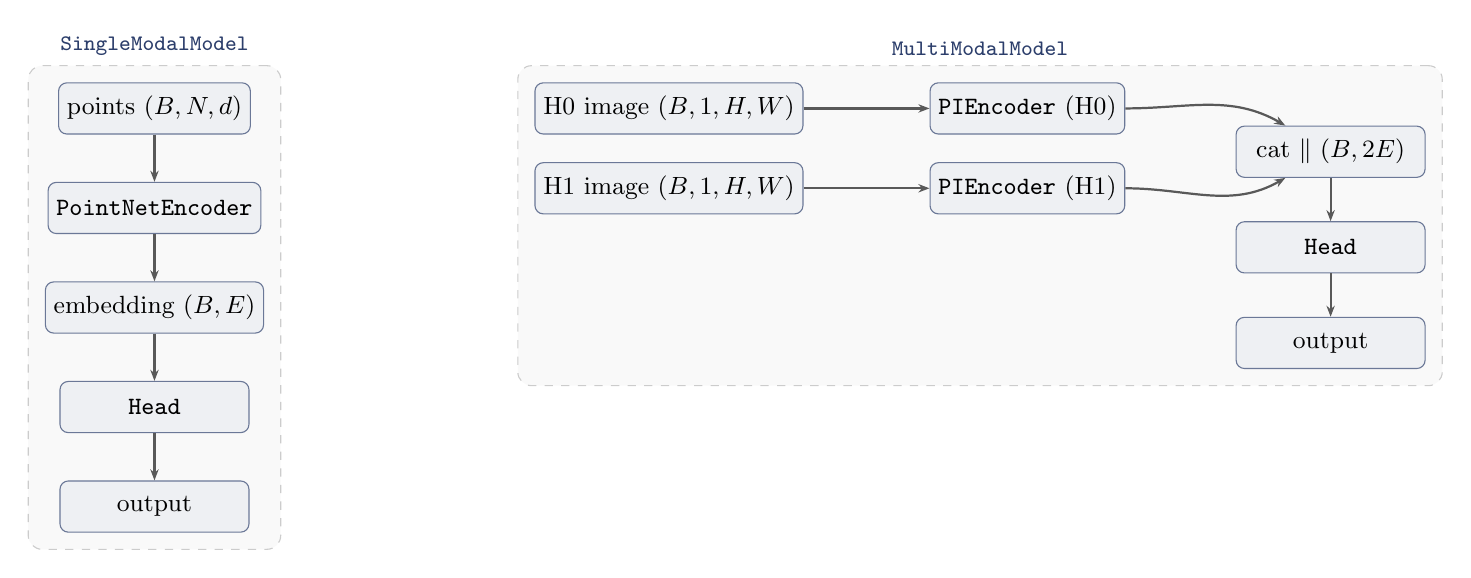
\begin{tikzpicture}[
  node distance=0.6cm and 2.2cm,
  every node/.style={font=\small},
  box/.style={rectangle, rounded corners=3pt,
              draw=headercol!70, fill=headercol!8,
              minimum height=0.65cm, minimum width=2.4cm,
              text centered, inner sep=3pt},
  arr/.style={-{Stealth[length=4pt]}, thick, gray!70!black},
  grp/.style={draw=gray!40, dashed, rounded corners=5pt,
              fill=gray!5, inner sep=6pt},
]

%% Single modal (left column)
\node[box] (pc_in)  {points $(B, N, d)$};
\node[box, below=of pc_in]  (pne)   {\texttt{PointNetEncoder}};
\node[box, below=of pne]    (emb1)  {embedding $(B, E)$};
\node[box, below=of emb1]   (hd1)   {\texttt{Head}};
\node[box, below=of hd1]    (out1)  {output};

\draw[arr] (pc_in) -- (pne);
\draw[arr] (pne)   -- (emb1);
\draw[arr] (emb1)  -- (hd1);
\draw[arr] (hd1)   -- (out1);

\begin{scope}[on background layer]
  \node[grp, fit=(pc_in)(pne)(emb1)(hd1)(out1),
        label={[font=\footnotesize\bfseries, text=headercol]above:
               \texttt{SingleModalModel}}] {};
\end{scope}

%% Multi modal (right column)
\node[box, right=3.6cm of pc_in] (pi0_in) {H0 image $(B,1,H,W)$};
\node[box, below=0.35cm of pi0_in] (pi1_in) {H1 image $(B,1,H,W)$};

\node[box, right=1.6cm of pi0_in] (enc0) {\texttt{PIEncoder} (H0)};
\node[box, right=1.6cm of pi1_in] (enc1) {\texttt{PIEncoder} (H1)};

\node[box, right=1.4cm of enc0, yshift=-0.55cm] (cat) {cat $\Vert$ $(B,2E)$};
\node[box, below=0.55cm of cat] (hd2)  {\texttt{Head}};
\node[box, below=0.55cm of hd2] (out2) {output};

\draw[arr] (pi0_in) -- (enc0);
\draw[arr] (pi1_in) -- (enc1);
\draw[arr] (enc0)   to[out=0, in=150] (cat);
\draw[arr] (enc1)   to[out=0, in=210] (cat);
\draw[arr] (cat)    -- (hd2);
\draw[arr] (hd2)    -- (out2);

\begin{scope}[on background layer]
  \node[grp, fit=(pi0_in)(pi1_in)(enc0)(enc1)(cat)(hd2)(out2),
        label={[font=\footnotesize\bfseries, text=headercol]above:
               \texttt{MultiModalModel}}] {};
\end{scope}

\end{tikzpicture}
\caption{Left: \texttt{SingleModalModel} with \texttt{PointNetEncoder}.
         Right: \texttt{MultiModalModel} fusing H0 and H1 persistence-image
         encoders via concatenation before the shared head.}
\label{fig:nn}
\end{figure}

\subsection{Training Utilities}

\subsubsection{\code{train\_val\_test\_split()}}
\pyfile{src/cloudforger/nn/splits.py}

\begin{lstlisting}
def train_val_test_split(
    dataset: Dataset,
    fractions: tuple[float, float, float] = (0.7, 0.15, 0.15),
    seed: int = 0,
) -> tuple[Subset, Subset, Subset]:
    # Splits randomly; fractions must sum to 1.
    # Remainder points (from rounding) go to the test split.
\end{lstlisting}

\subsubsection{\code{train\_one\_epoch()} and \code{evaluate()}}
\pyfile{src/cloudforger/nn/train.py}

\begin{lstlisting}
def train_one_epoch(
    model, loader: DataLoader,
    optimizer: torch.optim.Optimizer,
    loss_fn: nn.Module,
    device: torch.device,
) -> tuple[float, float]:
    # Sets model.train(), iterates loader.
    # Returns (avg_loss, accuracy) for the epoch.
    # Handles dict inputs for MultiModalModel via _to_device().

@torch.no_grad()
def evaluate(
    model, loader: DataLoader,
    loss_fn: nn.Module,
    device: torch.device,
) -> tuple[float, float]:
    # Sets model.eval(), no gradients.
    # Returns (avg_loss, accuracy).
\end{lstlisting}

Both functions handle both tensor and dict inputs transparently
via the internal \code{\_to\_device(inputs, device)} helper.
Accuracy is computed only for 1-D integer labels
(\code{argmax(logits) == labels}); for regression targets the
accuracy value is not meaningful.

\subsection{\code{standardize\_size()}}
\pyfile{src/cloudforger/core/utils.py}

\begin{lstlisting}
def standardize_size(cloud: PointCloud, n: int,
                     seed: int) -> PointCloud:
    # Raises ValueError if cloud.n_points < n.
    # Returns cloud unchanged if n_points == n.
    # Otherwise samples n points without replacement.
\end{lstlisting}

Used by the offline processing scripts to normalise cloud sizes before
saving datasets; not called by \code{PointCloudDataset} (which
subsamples on-the-fly per batch).

%% ═══════════════════════════════════════════════════════════════════════════
\section{Public API Quick Reference}
\label{sec:api}
%% ═══════════════════════════════════════════════════════════════════════════

\begin{longtable}{p{5.6cm} p{9.5cm}}
\toprule
\textbf{Callable} & \textbf{Description} \\
\midrule
\endhead
\bottomrule
\endfoot

\code{Box(low, high)} &
  Create an axis-aligned rectangular domain. \\[4pt]

\code{PoissonProcess(intensity)} &
  Homogeneous Poisson process; \code{intensity=None} gives the
  conditional (fixed-count) variant. \\[4pt]

\code{ThomasProcess(parent\_intensity,} \code{mean\_offspring, cluster\_scale)} &
  Clustered Neyman--Scott process with Gaussian offspring kernel. \\[4pt]

\code{MaternHardCoreProcess(parent\_intensity, hardcore\_radius)} &
  Repulsive hard-core process (Matérn Type II). \\[4pt]

\code{process.sample(n, region, seed)} &
  Public entry point for all processes.
  Returns a \code{PointCloud} with full provenance metadata. \\[4pt]

\code{standardize\_size(cloud, n, seed)} &
  Deterministically subsample a cloud to exactly \code{n} points. \\[4pt]

\code{RipsFiltration(maxdim, thresh)} &
  Configure a Rips filtration. \\[4pt]

\code{filtration.compute(cloud)} &
  Compute persistent homology; returns \code{PersistenceDiagram}. \\[4pt]

\code{PersistenceDiagram.finite\_pairs(dim)} &
  Extract birth--death pairs with finite death time. \\[4pt]

\code{calibrate(diagrams, percentiles)} &
  Pool statistics over a collection of diagrams; return percentile bounds
  for birth and persistence per dimension. \\[4pt]

\code{calibrate\_report(diagrams, percentiles)} &
  Human-readable version of \code{calibrate()}. \\[4pt]

\code{PersistenceImager(birth\_range, pers\_range,} \code{resolution, sigma, weight\_fn)} &
  Construct a fixed-resolution rasterizer for one homology dimension. \\[4pt]

\code{imager.transform(diagram, dim)} &
  Rasterize dimension \code{dim} of a diagram into a
  \code{(resolution, resolution)} float array. \\[4pt]

\code{MultiChannelImager(imagers)} &
  Bundle per-dimension imagers; produces \code{dict[int, ndarray]}. \\[4pt]

\code{multi.transform(diagram)} &
  Apply all configured imagers to a diagram. \\[4pt]

\code{PairDistanceCDF(n\_samples, grid\_size)} &
  Pair-distance empirical CDF statistic. \\[4pt]

\code{statistic.compute(cloud)} &
  Compute the ECDF vector; returns 1-D float array of length
  \code{grid\_size}. \\[4pt]

\code{PointCloudDataset(clouds, labels, n\_points)} &
  PyTorch \code{Dataset} over raw point clouds. \\[4pt]

\code{PersistenceImageDataset(images, labels)} &
  PyTorch \code{Dataset} over persistence-image dicts. \\[4pt]

\code{CorrelationFeatureDataset(features, labels,} \code{statistic\_names)} &
  PyTorch \code{Dataset} over correlation-feature vectors. \\[4pt]

\code{PointNetEncoder(input\_dim, embedding\_dim,} \code{hidden\_dims)} &
  PointNet backbone for raw point clouds. \\[4pt]

\code{PIEncoder(in\_channels, embedding\_dim)} &
  CNN encoder for persistence images. \\[4pt]

\code{StatsEncoder(input\_dim, embedding\_dim,} \code{hidden\_dims)} &
  MLP encoder for flat feature vectors. \\[4pt]

\code{ClassificationHead(embedding\_dim,} \code{n\_classes, hidden\_dims, dropout)} &
  MLP head producing class logits. \\[4pt]

\code{ParameterEstimator(embedding\_dim,} \code{n\_params, hidden\_dims, dropout)} &
  MLP head producing real-valued regression targets. \\[4pt]

\code{SingleModalModel(encoder, head)} &
  Composes one encoder with one head. \\[4pt]

\code{MultiModalModel(encoders, head)} &
  Late-fusion model: concatenates embeddings from multiple encoders. \\[4pt]

\code{train\_val\_test\_split(dataset, fractions, seed)} &
  Reproducible random split into train/val/test subsets. \\[4pt]

\code{train\_one\_epoch(model, loader,} \code{optimizer, loss\_fn, device)} &
  One full pass over a \code{DataLoader}; returns (loss, accuracy). \\[4pt]

\code{evaluate(model, loader, loss\_fn, device)} &
  Evaluation pass (no gradients); returns (loss, accuracy). \\[4pt]

\end{longtable}

%% ═══════════════════════════════════════════════════════════════════════════
\section{Usage Walkthrough}
\label{sec:walkthrough}
%% ═══════════════════════════════════════════════════════════════════════════

This section shows the minimal code needed to go from nothing to a
trained single-modal classifier, using the TDA pathway.
The example is self-contained and can be run directly after installing
the package dependencies.

\subsection{Step 1: Generate Clouds}

\begin{lstlisting}
import numpy as np
from cloudforger.core.region import Box
from cloudforger.processes.poisson import PoissonProcess
from cloudforger.processes.thomas import ThomasProcess
from cloudforger.processes.matern import MaternHardCoreProcess

region = Box(low=np.zeros(2), high=np.ones(2))

# Three processes, 100 clouds each
processes = [
    (PoissonProcess(),                                label := 0),
    (ThomasProcess(parent_intensity=20.0,
                   mean_offspring=10.0,
                   cluster_scale=0.05),               label := 1),
    (MaternHardCoreProcess(parent_intensity=2000.0,
                           hardcore_radius=0.02),     label := 2),
]

clouds, labels = [], []
for proc, lbl in [
    (PoissonProcess(),                              0),
    (ThomasProcess(20.0, 10.0, 0.05),              1),
    (MaternHardCoreProcess(2000.0, 0.02),           2),
]:
    for seed in range(100):
        cloud = proc.sample(n=500, region=region, seed=seed)
        clouds.append(cloud)
        labels.append(lbl)

labels = np.array(labels)
\end{lstlisting}

\subsection{Step 2: Compute Persistence Diagrams}

\begin{lstlisting}
from cloudforger.tda.filtration.rips import RipsFiltration

filt = RipsFiltration(maxdim=1)
diagrams = [filt.compute(c) for c in clouds]
\end{lstlisting}

\subsection{Step 3: Calibrate and Vectorize}

\begin{lstlisting}
from cloudforger.tda.calibration import calibrate
from cloudforger.tda.vectorizer.persistence_image import PersistenceImager
from cloudforger.tda.vectorizer.multi_channel import MultiChannelImager

stats = calibrate(diagrams, percentiles=(99.0,))

imagers = {}
for dim in [0, 1]:
    b_hi = stats[dim]["birth"][99.0]
    p_hi = stats[dim]["persistence"][99.0]
    imagers[dim] = PersistenceImager(
        birth_range=(0.0, b_hi),
        pers_range=(0.0, p_hi),
        resolution=64,
        sigma=0.01,
    )

mc = MultiChannelImager(imagers)
images = [mc.transform(d) for d in diagrams]
# images[i] == {0: ndarray(64,64), 1: ndarray(64,64)}
\end{lstlisting}

\subsection{Step 4: Build Datasets and Splits}

\begin{lstlisting}
import torch
from torch.utils.data import DataLoader
from cloudforger.nn.data import PersistenceImageDataset
from cloudforger.nn.splits import train_val_test_split

dataset = PersistenceImageDataset(images, labels)
train_ds, val_ds, test_ds = train_val_test_split(
    dataset, fractions=(0.7, 0.15, 0.15), seed=0
)

train_loader = DataLoader(train_ds, batch_size=32, shuffle=True)
val_loader   = DataLoader(val_ds,   batch_size=64)
test_loader  = DataLoader(test_ds,  batch_size=64)
\end{lstlisting}

\subsection{Step 5: Assemble and Train a Model}

\begin{lstlisting}
import torch.nn as nn
from cloudforger.nn.encoders.persistence_image import PIEncoder
from cloudforger.nn.models.multi_modal import MultiModalModel
from cloudforger.nn.heads.classifier import ClassificationHead
from cloudforger.nn.train import train_one_epoch, evaluate

device = torch.device("cuda" if torch.cuda.is_available() else "cpu")

# One encoder per homology dimension
encoders = {
    "h0": PIEncoder(in_channels=1, embedding_dim=128),
    "h1": PIEncoder(in_channels=1, embedding_dim=128),
}
head  = ClassificationHead(
    embedding_dim=256,   # 128 + 128
    n_classes=3,
    hidden_dims=(128,),
    dropout=0.1,
)
model = MultiModalModel(encoders=encoders, head=head).to(device)

optimizer = torch.optim.Adam(model.parameters(), lr=1e-3)
loss_fn   = nn.CrossEntropyLoss()

best_val = float("inf")
for epoch in range(50):
    tr_loss, tr_acc = train_one_epoch(
        model, train_loader, optimizer, loss_fn, device)
    vl_loss, vl_acc = evaluate(
        model, val_loader, loss_fn, device)
    if vl_loss < best_val:
        best_val = vl_loss
        torch.save(model.state_dict(), "best_model.pt")
    if (epoch + 1) % 10 == 0:
        print(f"Epoch {epoch+1:3d}: "
              f"train acc={tr_acc:.3f}  val acc={vl_acc:.3f}")

# Reload best and evaluate on test set
model.load_state_dict(torch.load("best_model.pt"))
te_loss, te_acc = evaluate(model, test_loader, loss_fn, device)
print(f"Test accuracy: {te_acc:.4f}")
\end{lstlisting}

%% ═══════════════════════════════════════════════════════════════════════════
\section{Known Ambiguities and Implementation Notes}
\label{sec:ambiguities}
%% ═══════════════════════════════════════════════════════════════════════════

\begin{enumerate}

  \item \textbf{\code{PIEncoder} default \code{in\_channels=2}.}
        The dataset always produces 1-channel images
        (\code{unsqueeze(0)}).
        The default of 2 targets a use case where H0 and H1 images
        are stacked before a \emph{single} encoder, but this is not
        wired up anywhere in the current runners.
        Use \code{in\_channels=1} when pairing with
        \code{PersistenceImageDataset}.

  \item \textbf{\code{PointProcess.sample()} and the \code{n} parameter.}
        For \code{ThomasProcess} and \code{MaternHardCoreProcess},
        \code{n} is passed to \code{\_sample\_points} but ignored ---
        the output count is always random.
        Callers should not rely on exact counts from these processes;
        use \code{standardize\_size()} or calibrate the parent intensity
        to achieve the desired expected count.

  \item \textbf{Matérn thinning loop.}
        The thinning in \code{MaternHardCoreProcess.\_sample\_points}
        uses a Python-level loop over all parents.
        For large parent intensities (many thousands of points) this
        is the performance bottleneck.

  \item \textbf{Persistence imager clipping.}
        Gaussian kernels are evaluated for all pairs, including those
        outside \code{birth\_range} / \code{pers\_range}.
        Out-of-range pairs still contribute tails to in-range pixels.
        This matches the spirit of the Adams et al.\ persistence image
        definition but can cause mild boundary effects near the image
        edges.

  \item \textbf{Module naming discrepancy.}
        Some file-level comments and the \code{train.py} module header
        reference the name \code{pointforge} (the older package name)
        rather than \code{cloudforger}.
        The public import paths use \code{cloudforger} throughout;
        the stale comments are cosmetic.

  \item \textbf{Parameter estimation accuracy metric.}
        \code{train\_one\_epoch} and \code{evaluate} compute accuracy
        via \code{argmax(logits) == labels}, which is only meaningful
        for integer class labels.
        When using \code{ParameterEstimator}, the returned accuracy
        is meaningless and should be ignored; log the raw loss instead.

\end{enumerate}

\end{document}
